\clearpage
\section{Appendix}

\subsection{Figures}

\begin{figure}[!h]
    \centering
    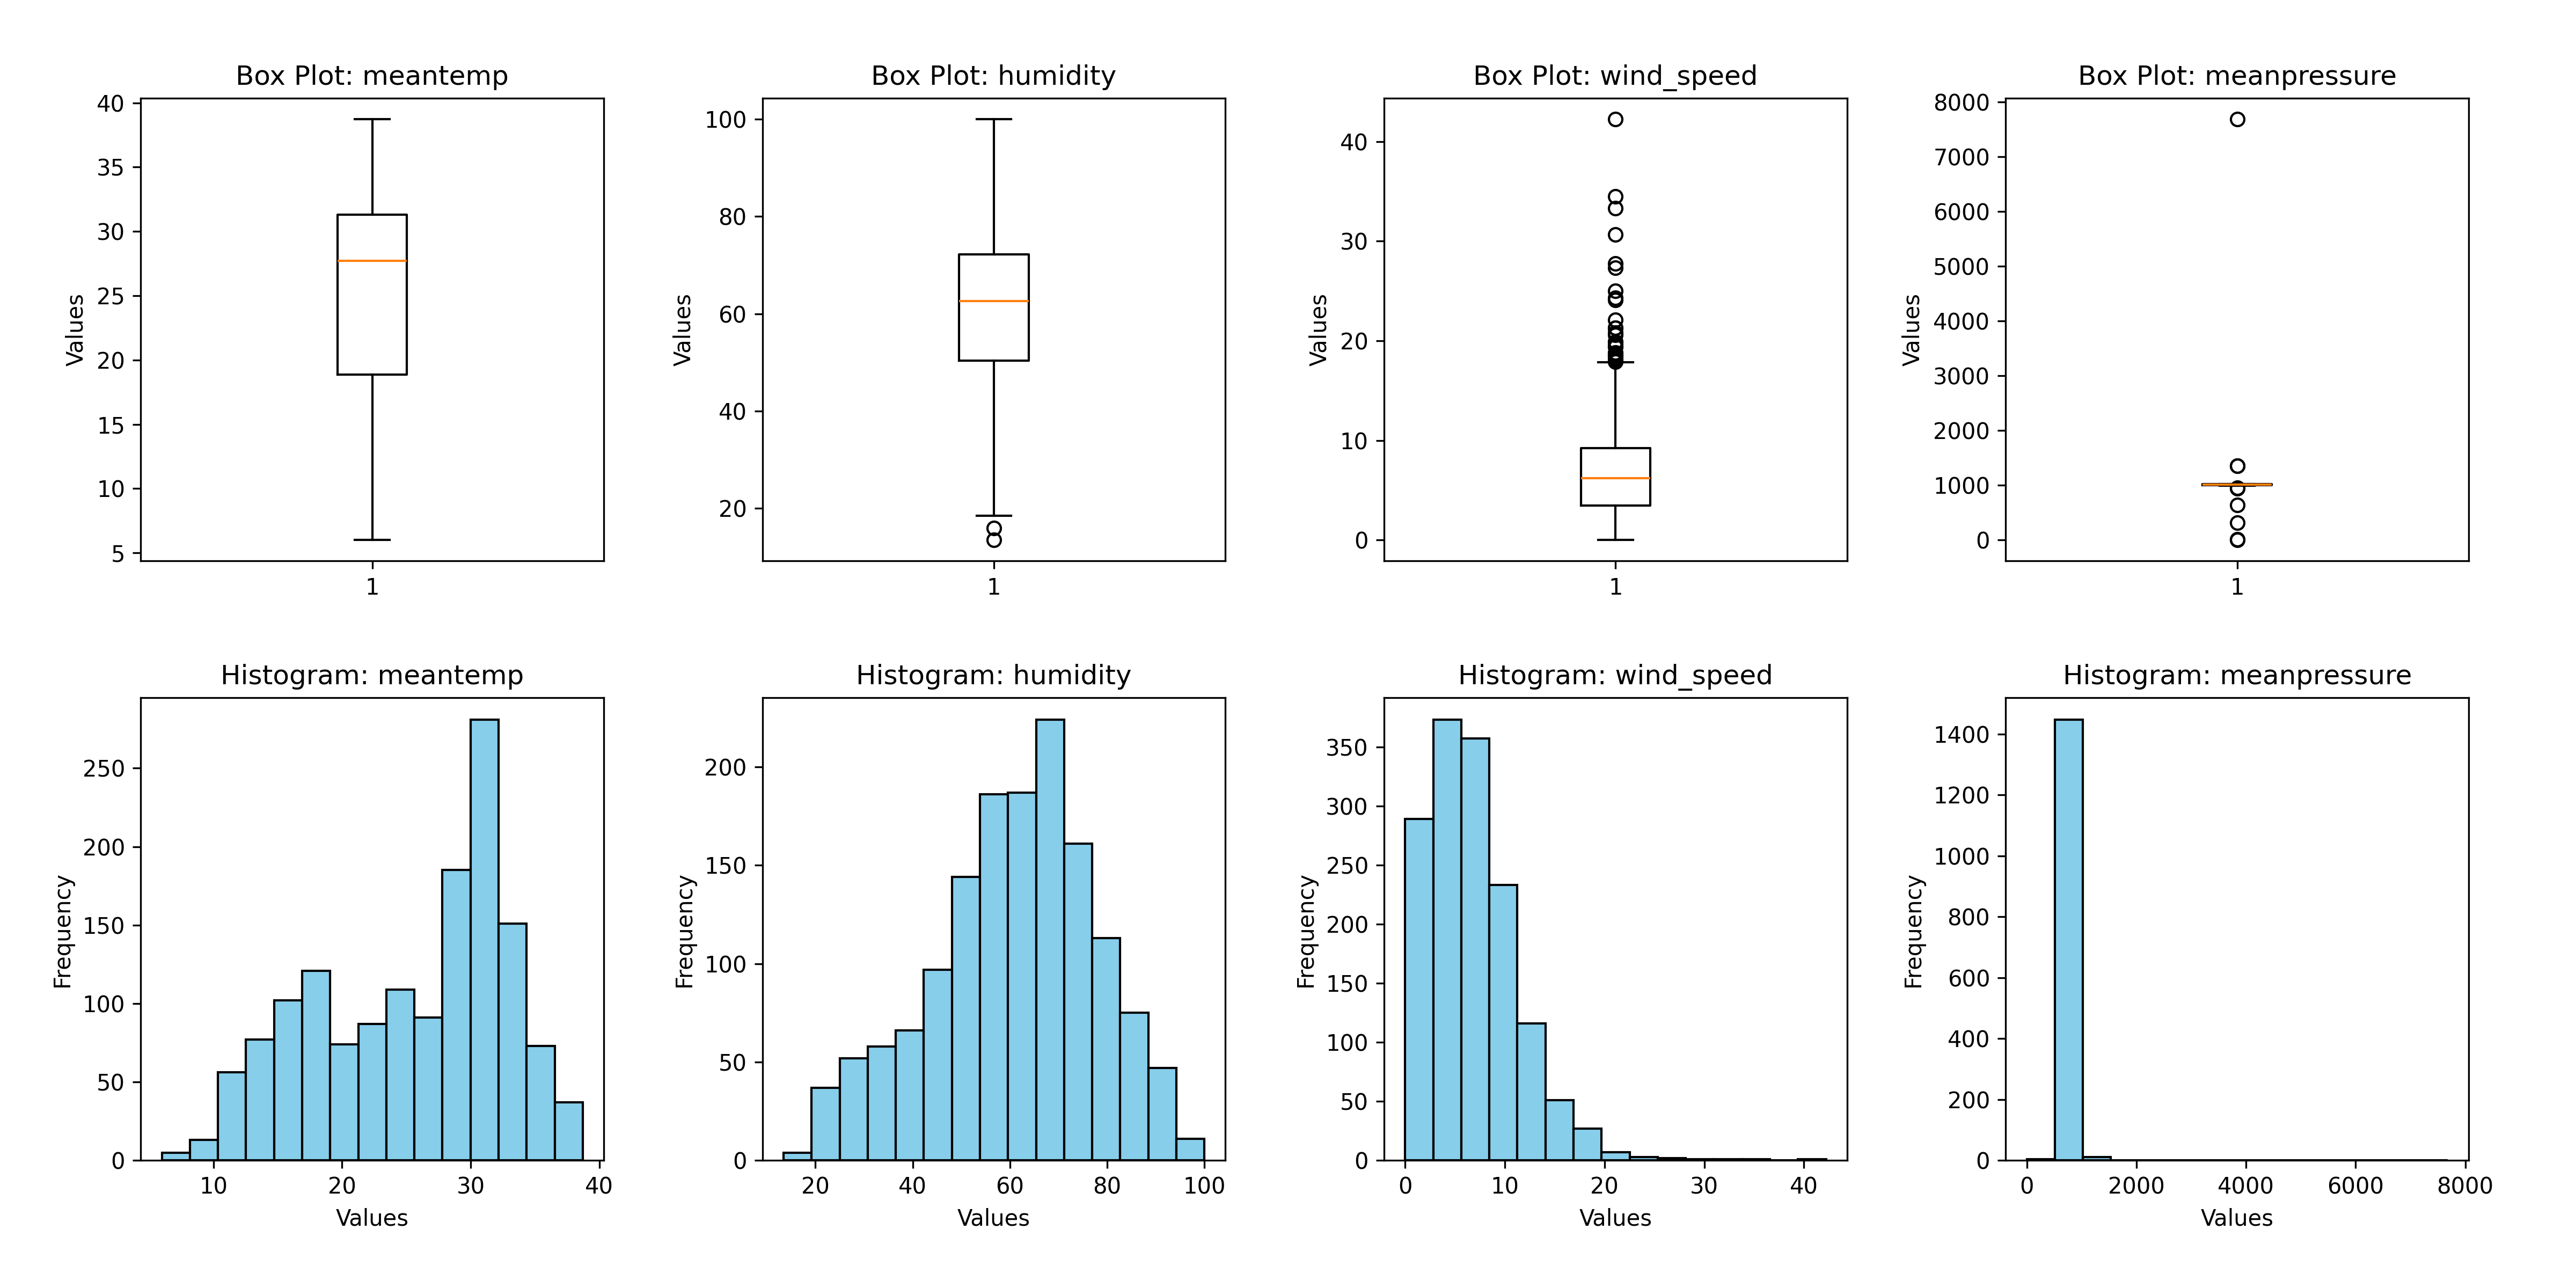
\includegraphics[width=.8\textwidth]{images/raw_train_data.png}
    \caption{\small \textit{Distribution of the raw data without replacing outliers}}
    \label{fig:figure1}
\end{figure}

\begin{figure}[!h]
    \centering
    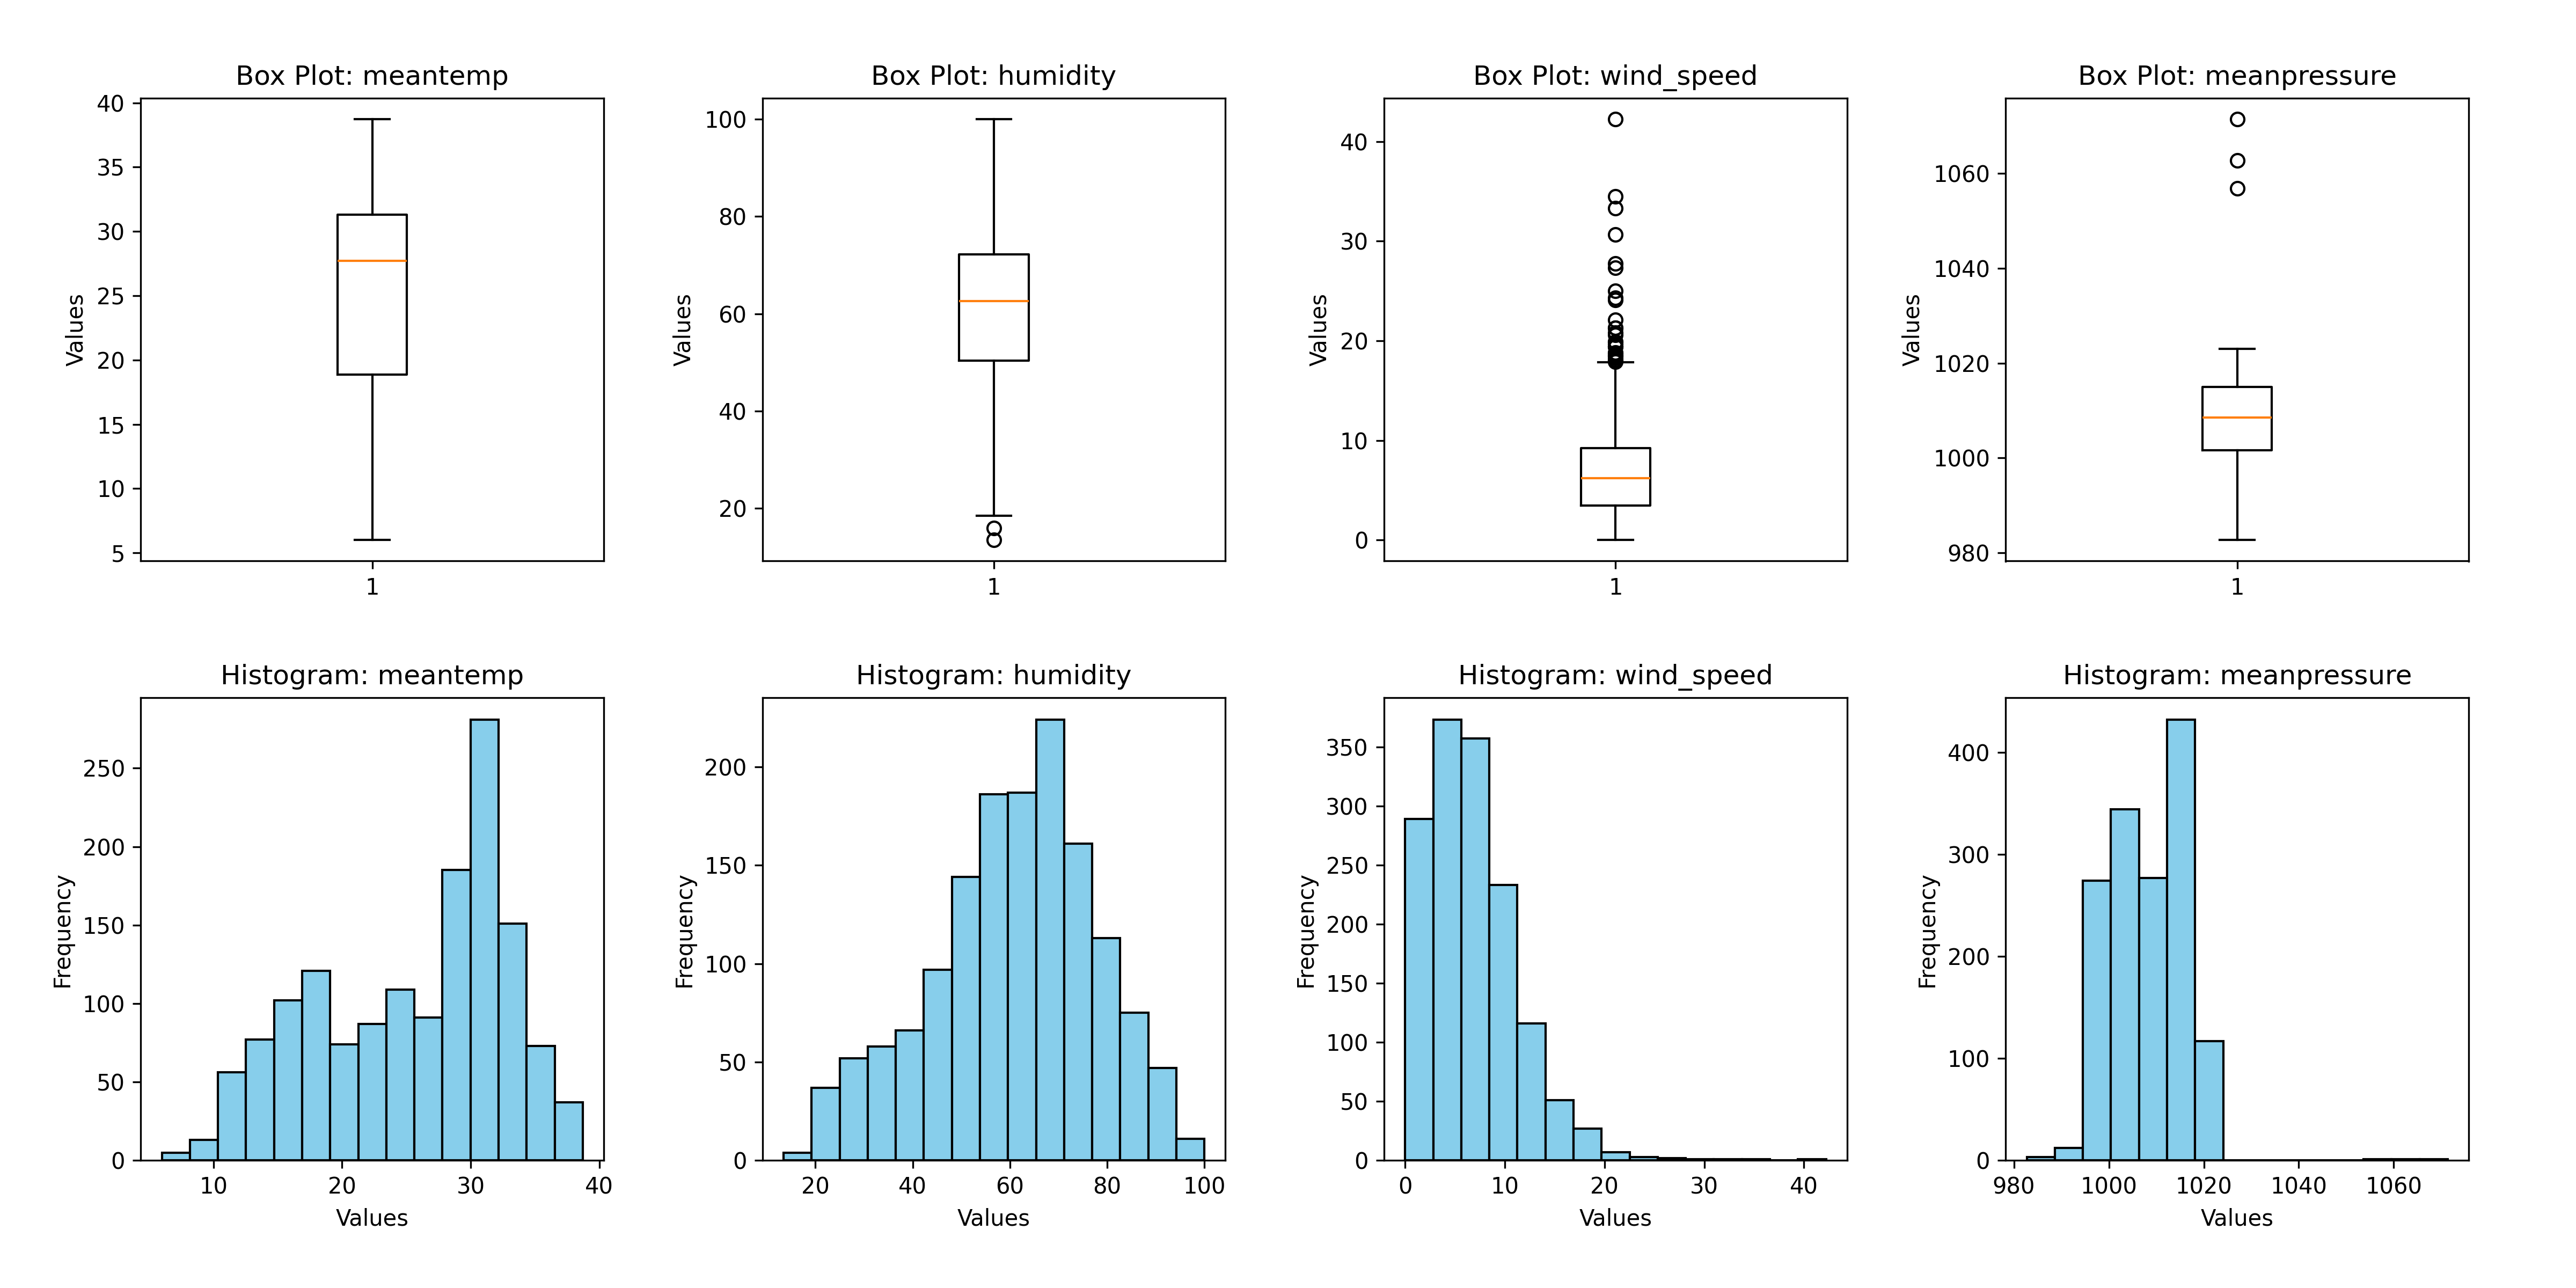
\includegraphics[width=.8\textwidth]{images/processed_train_data_box_and_hist_plots.png}
    \caption{\small \textit{Distribution of the processed data after replacing outliers}}
    \label{fig:figure1}
\end{figure}

\begin{figure}[!h]
    \centering
    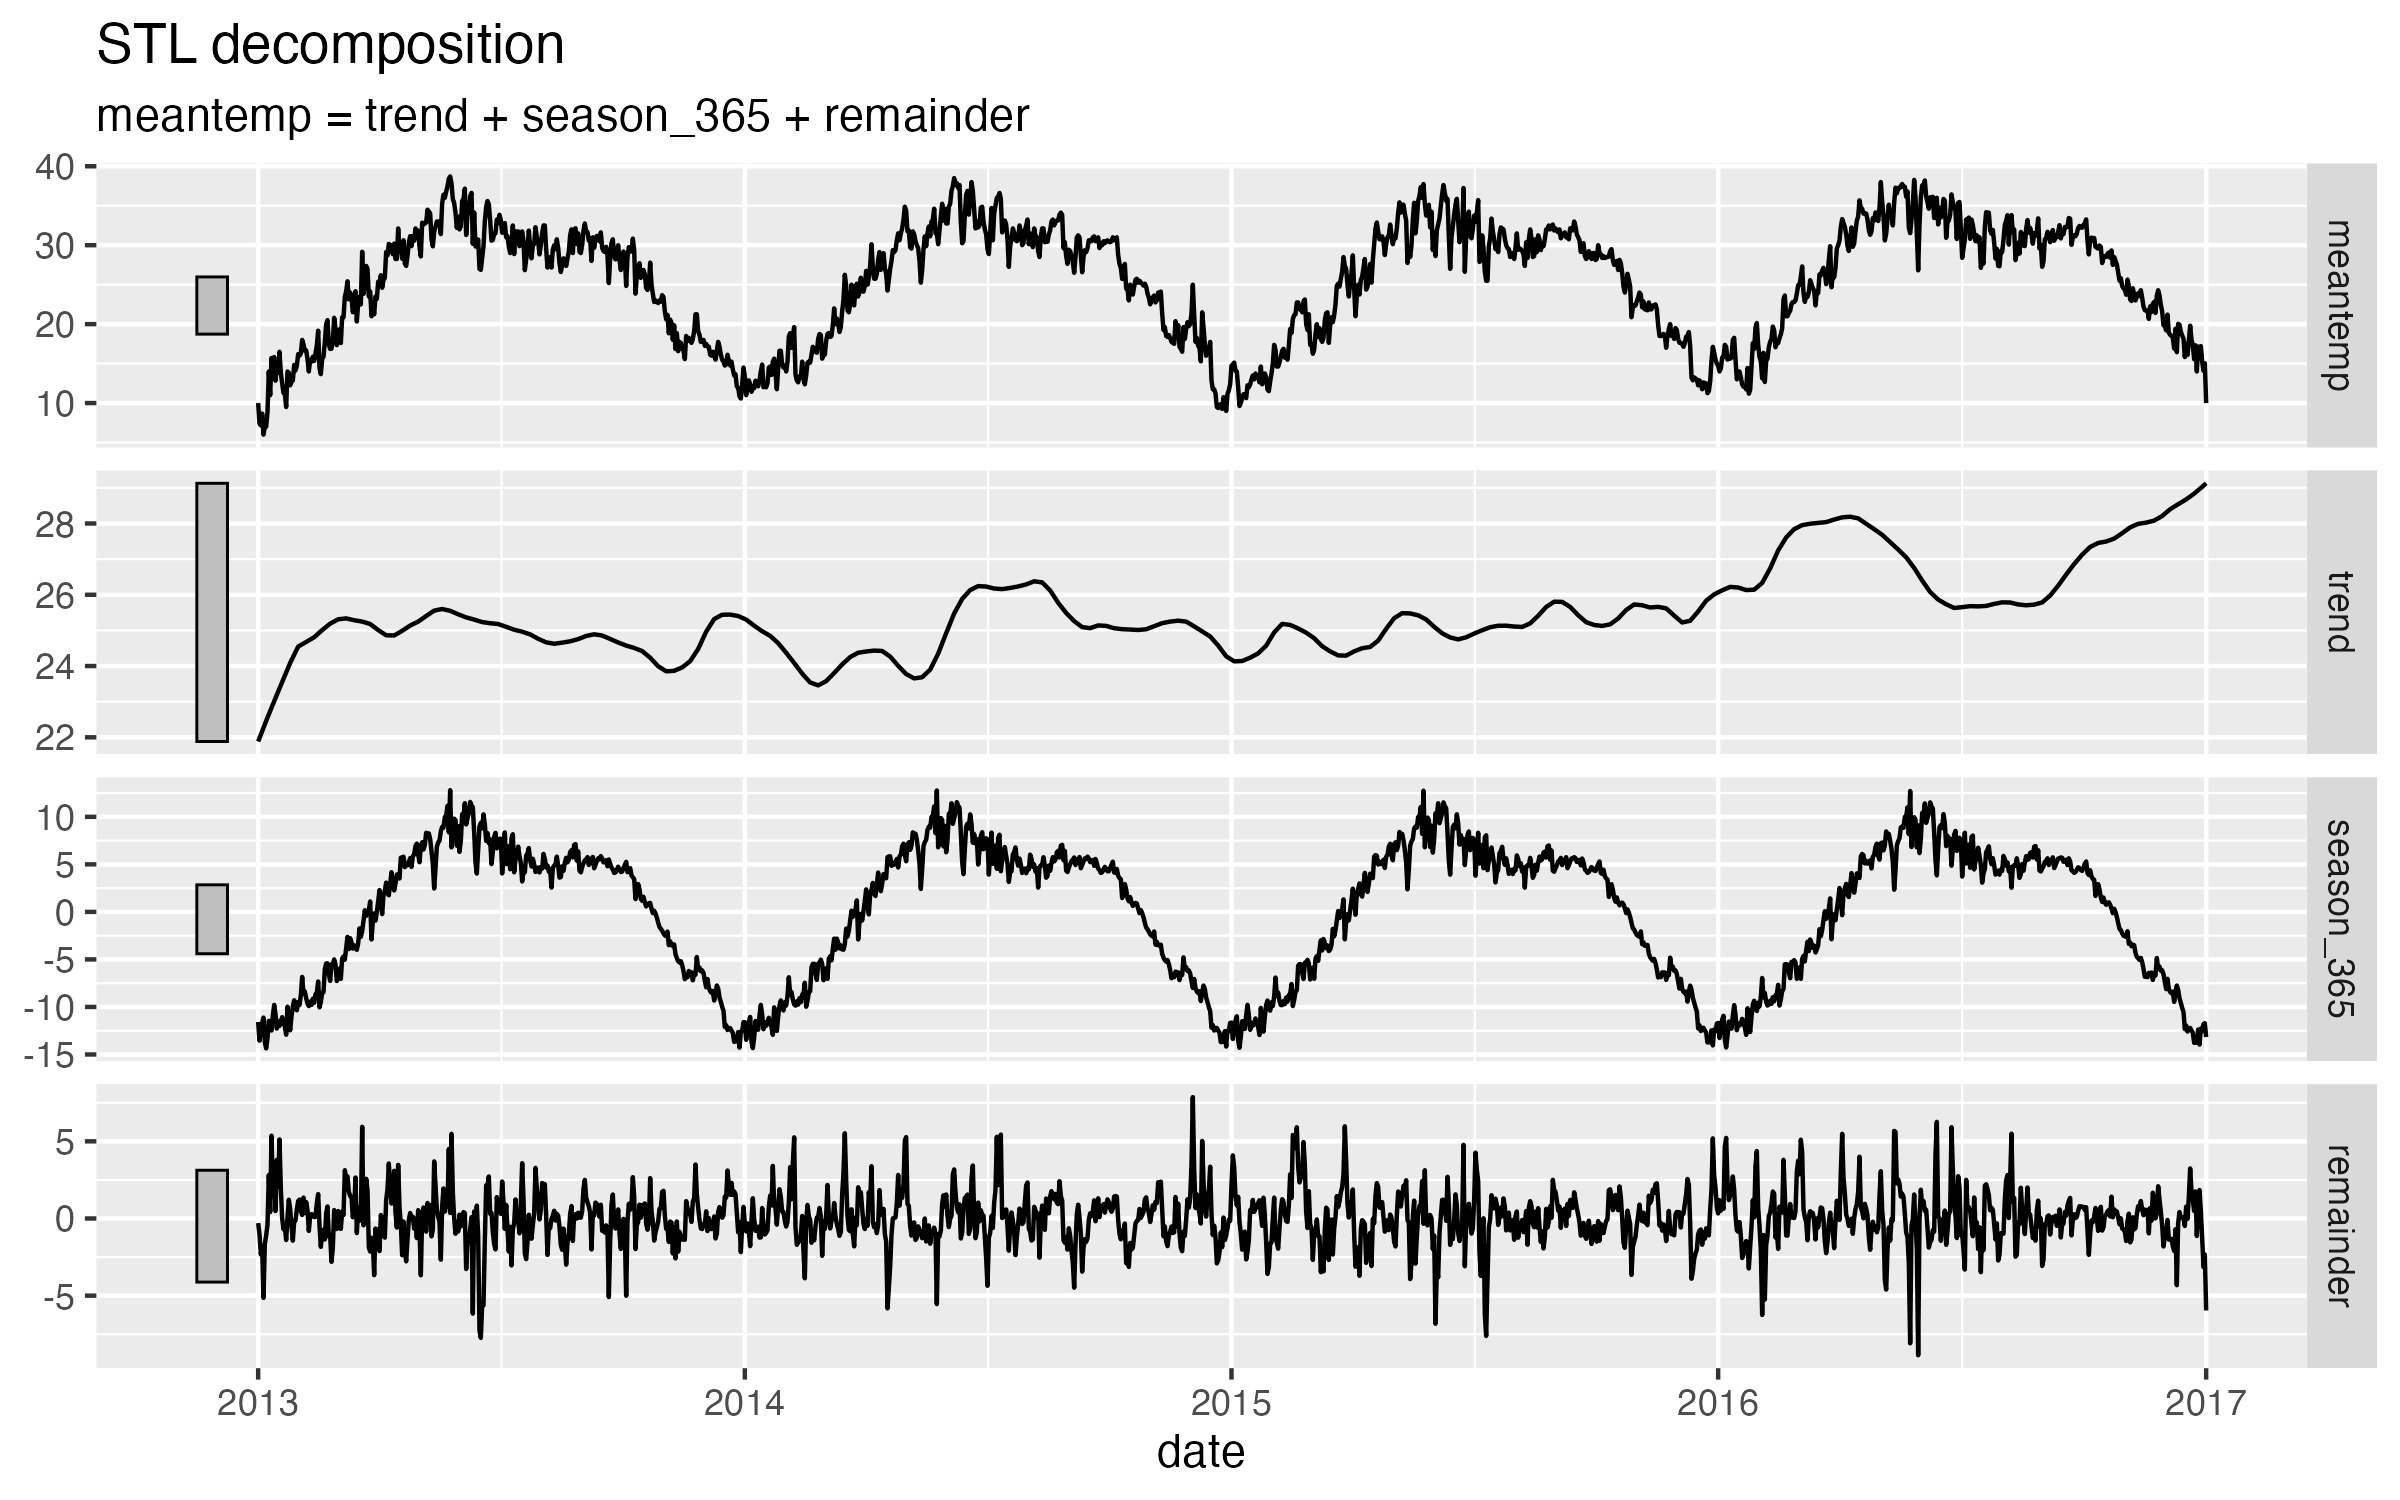
\includegraphics[width=.8\textwidth]{images/decomposition_plot.png}
    \caption{\small \textit{STL Decomposition of the mean temperature variable 
    (pointing period = 365 days)}}
    \label{fig:figure1}
\end{figure}

\begin{figure}[!h]
    \centering
    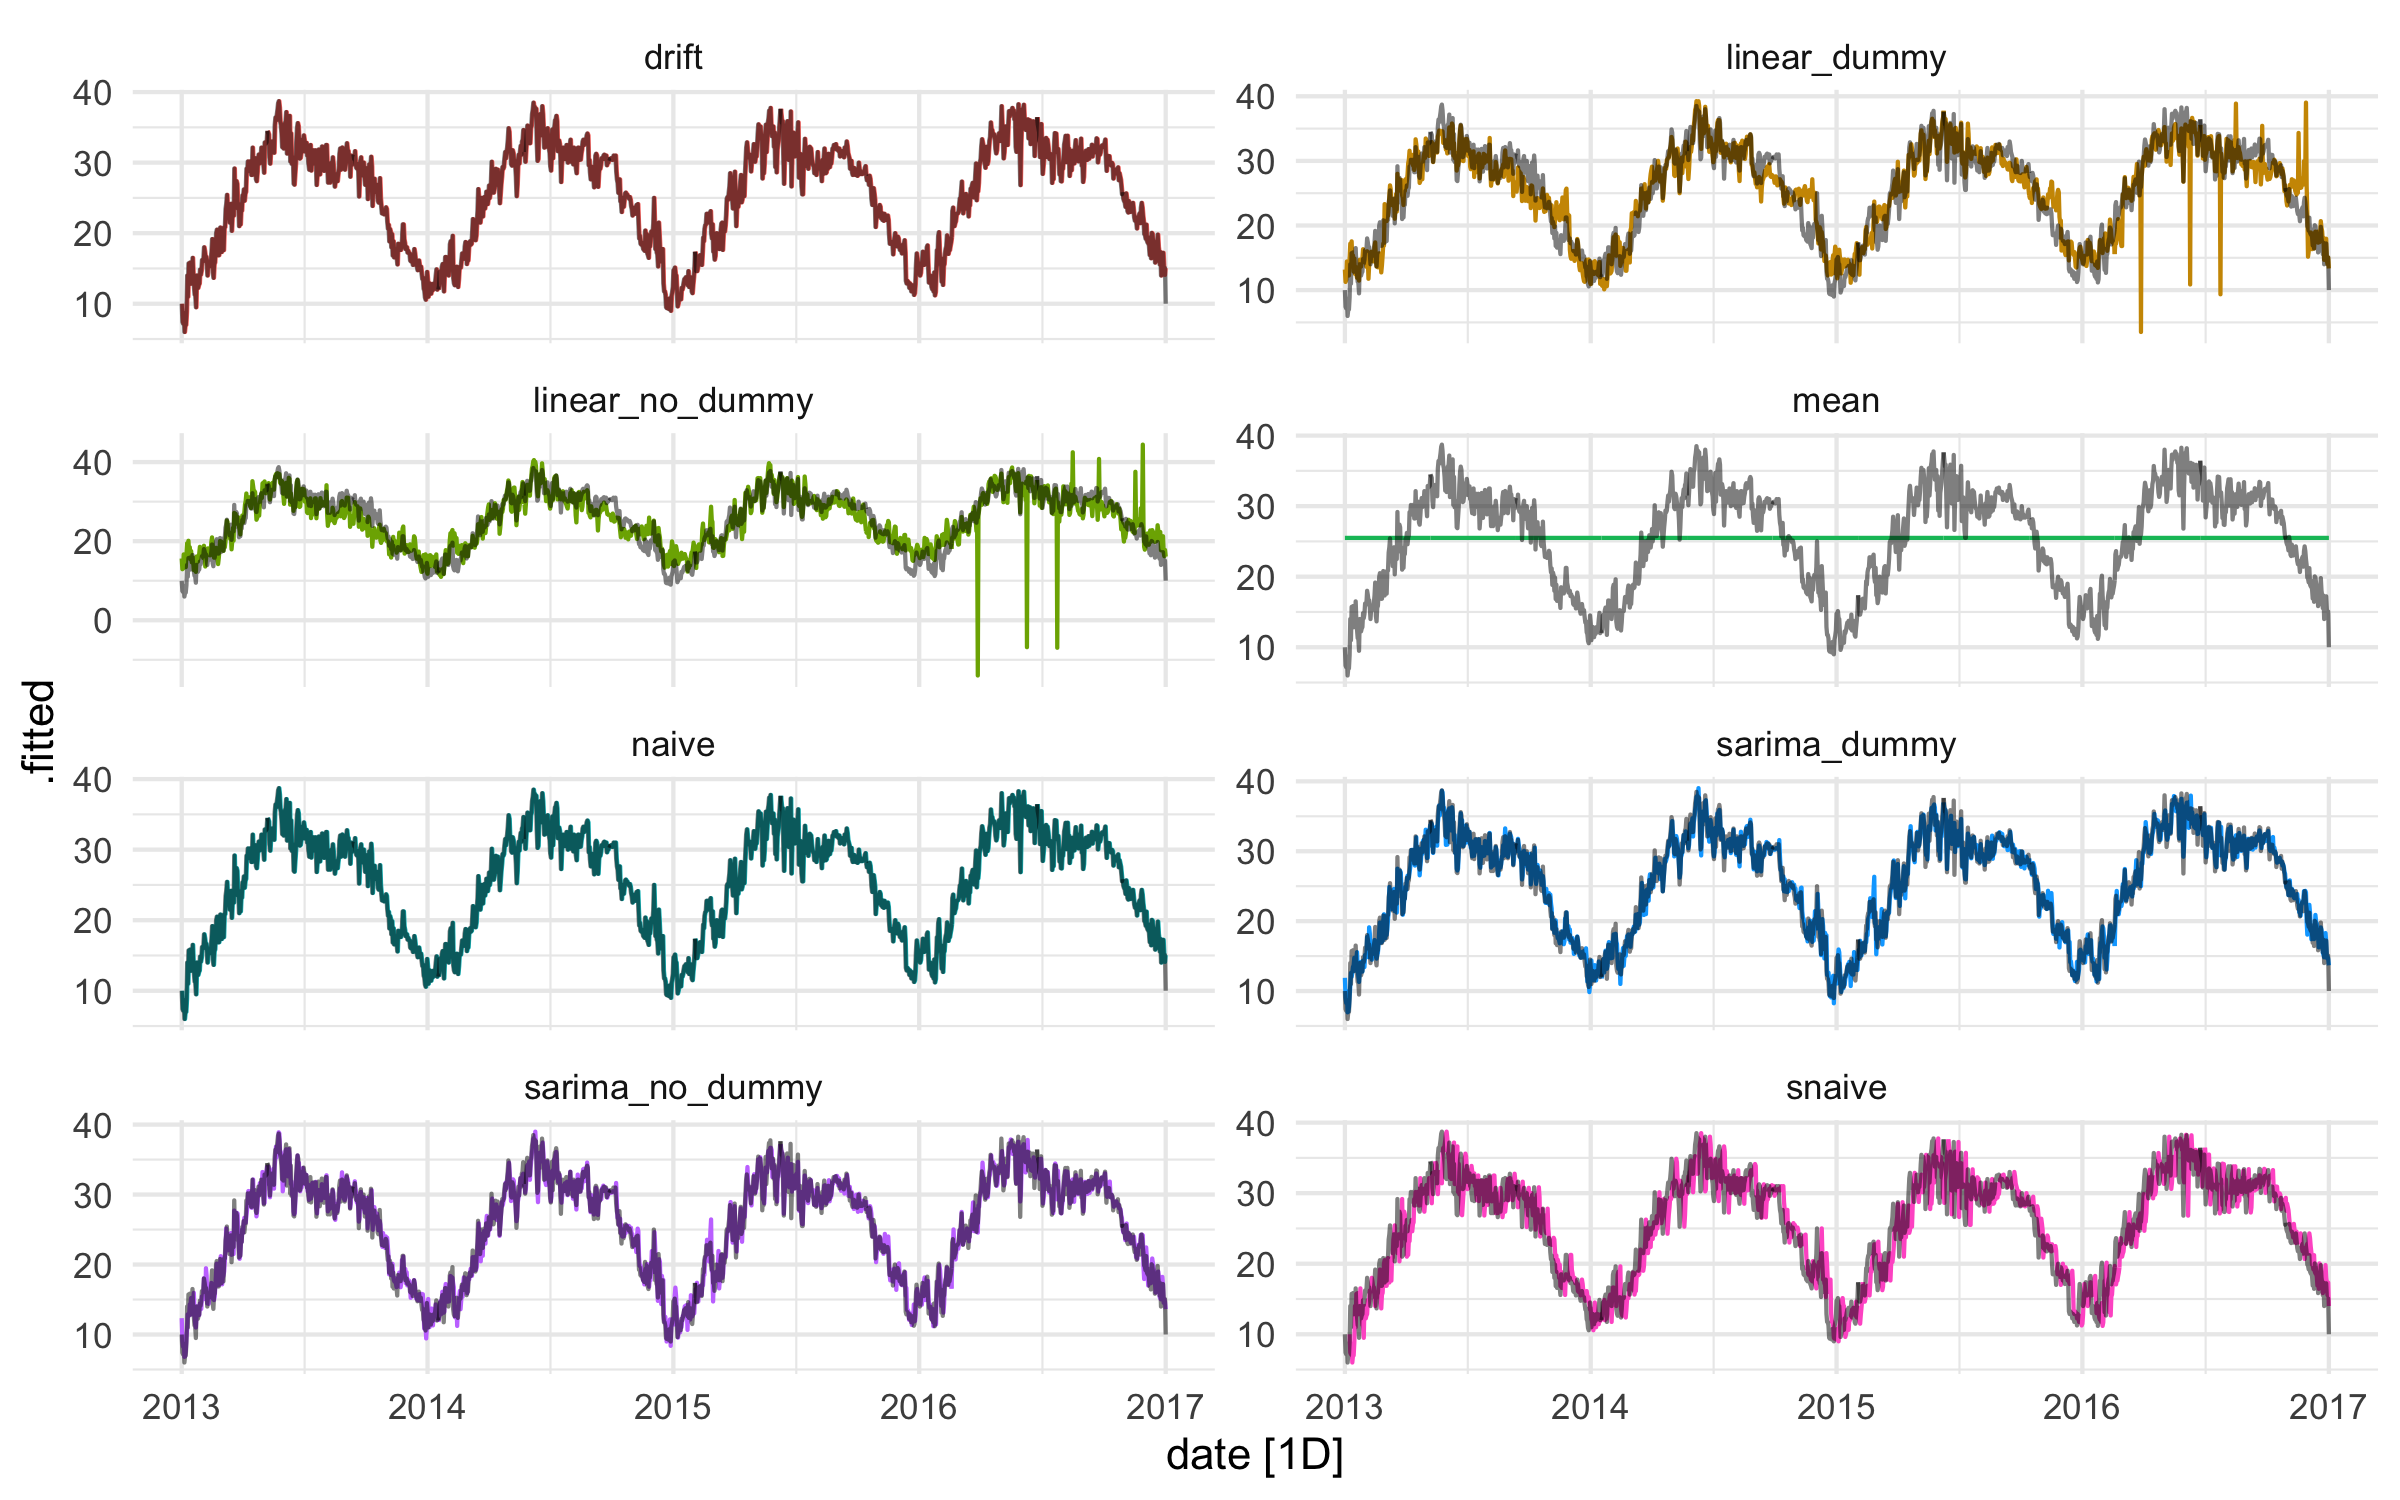
\includegraphics[width=.8\textwidth]{images/fitted_values_all_models.png}
    \caption{\small \textit{Fitted values and the true values on training data}}
    \label{fig:figure1}
\end{figure}

\begin{figure}[!h]
    \centering
    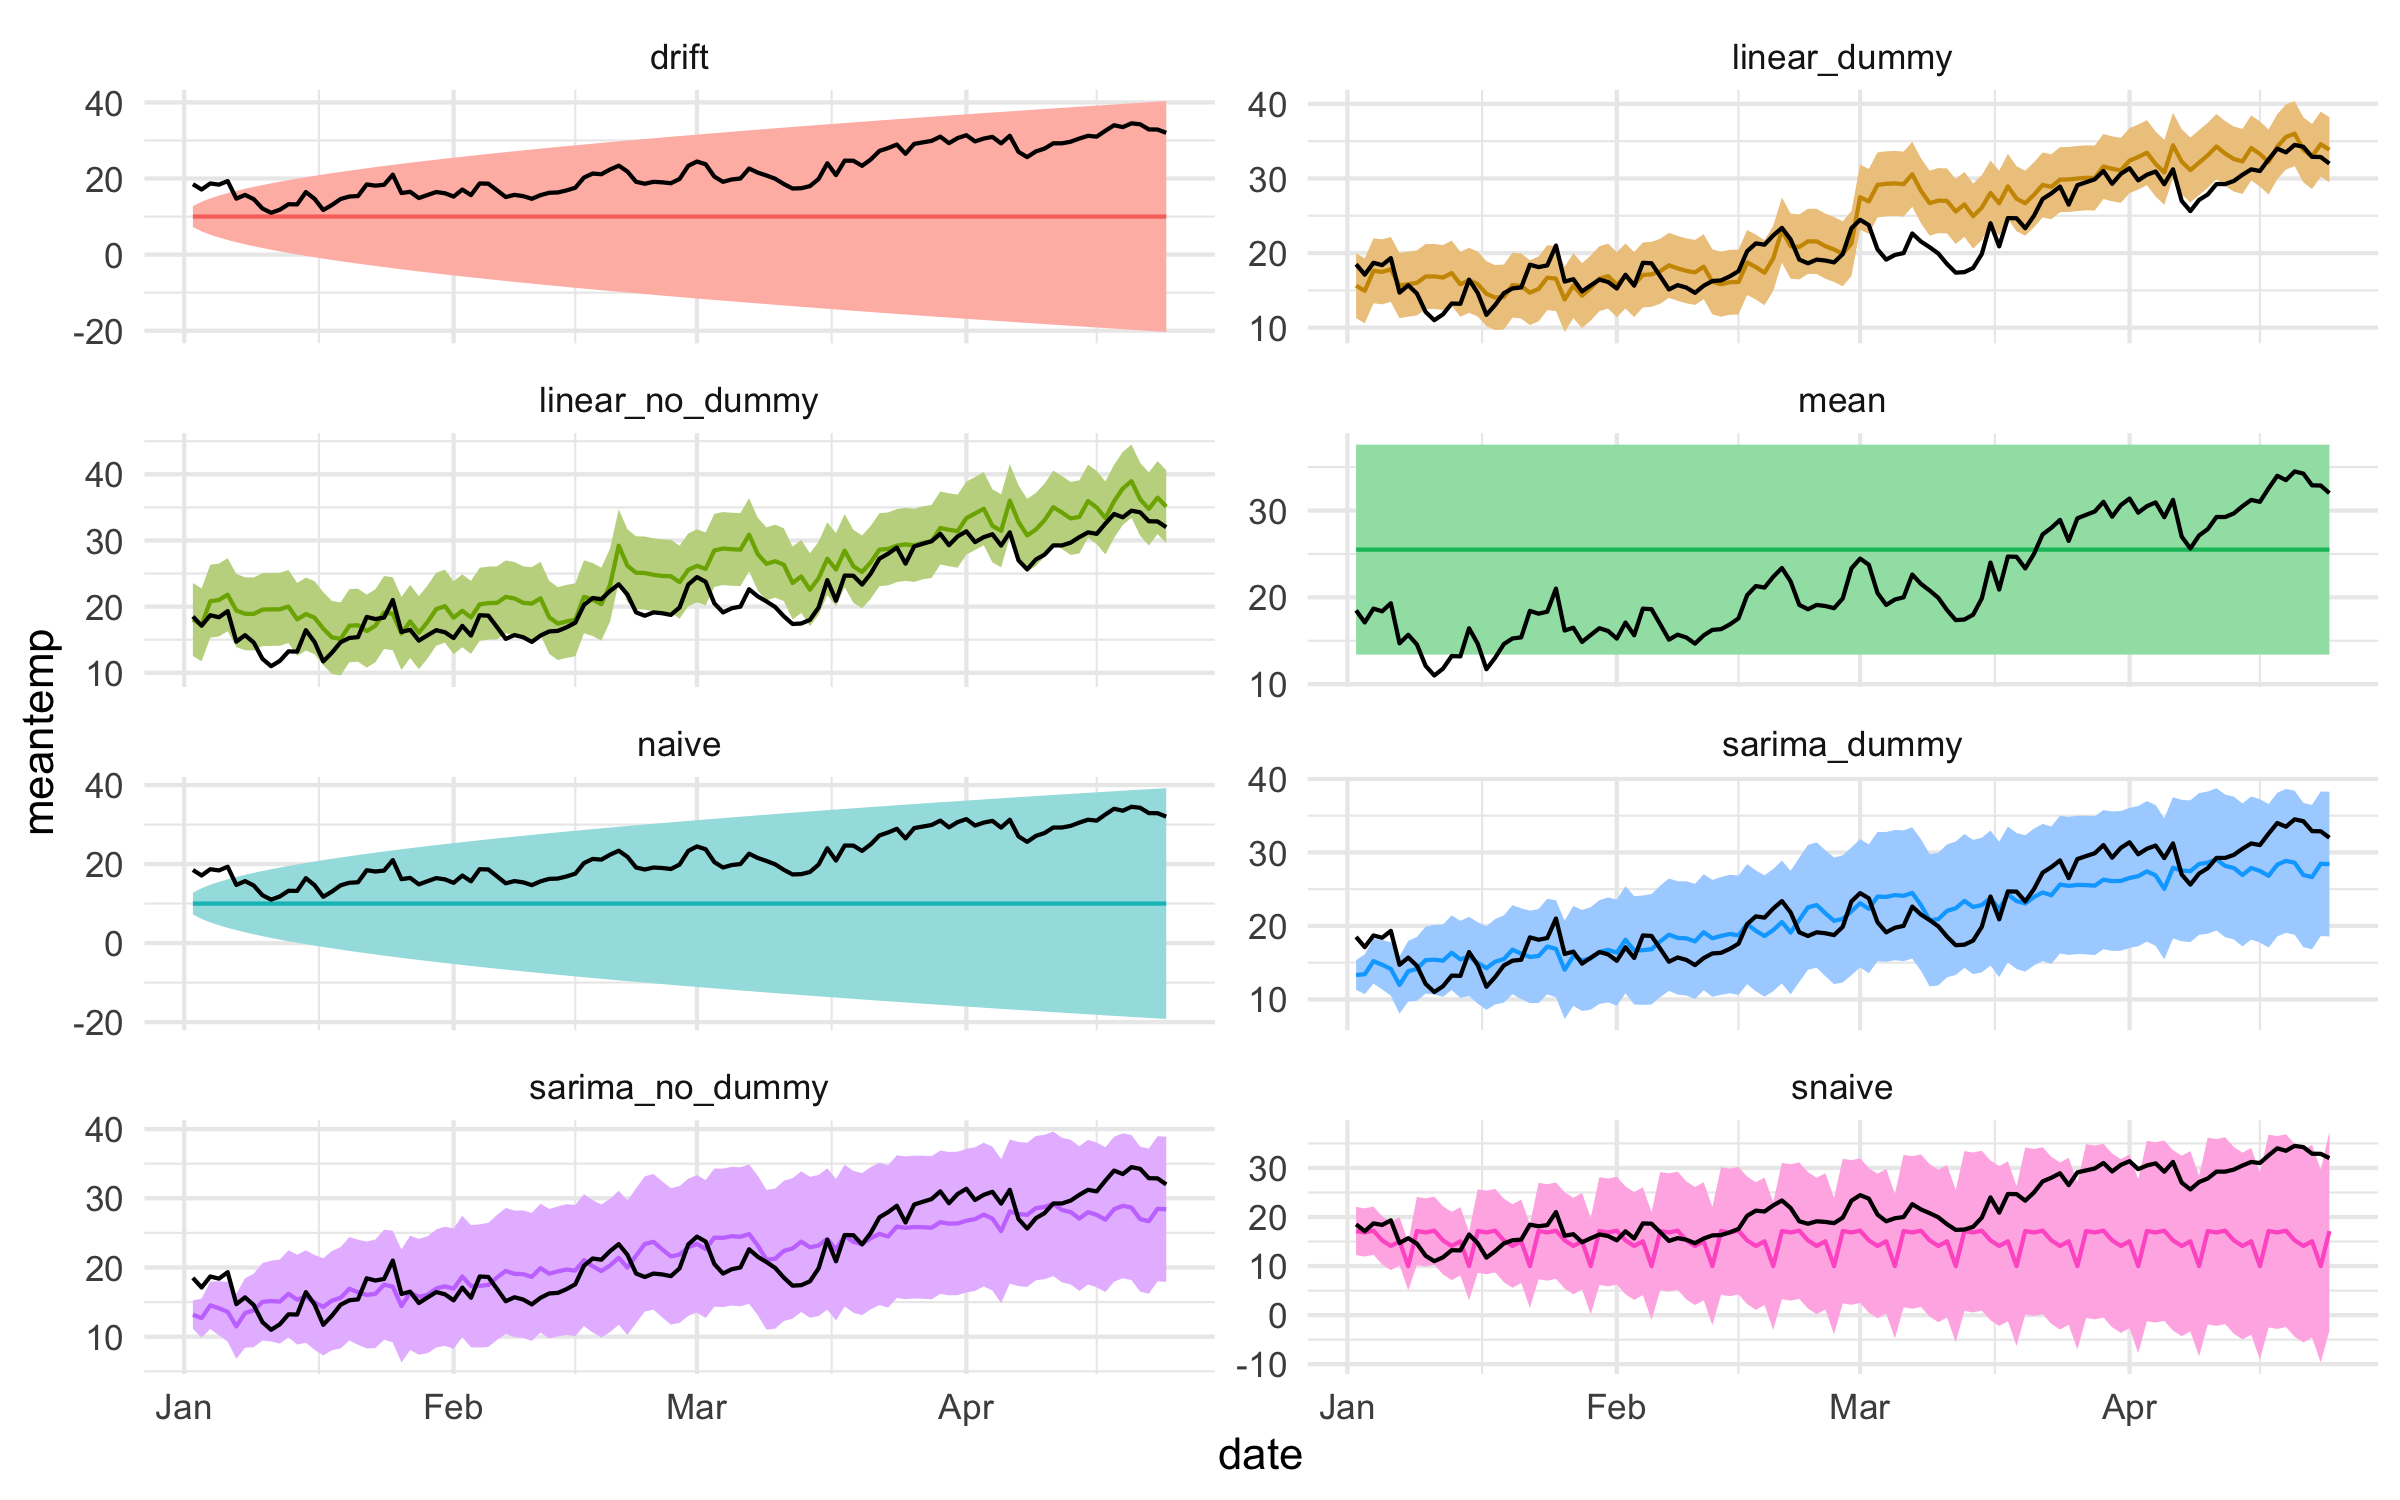
\includegraphics[width=.8\textwidth]{images/forecasts_CI90.png}
    \caption{\small \textit{Forecasts with 90\% confidence interval of all models}}
    \label{fig:figure1}
\end{figure}

\begin{figure}[!h]
    \centering
    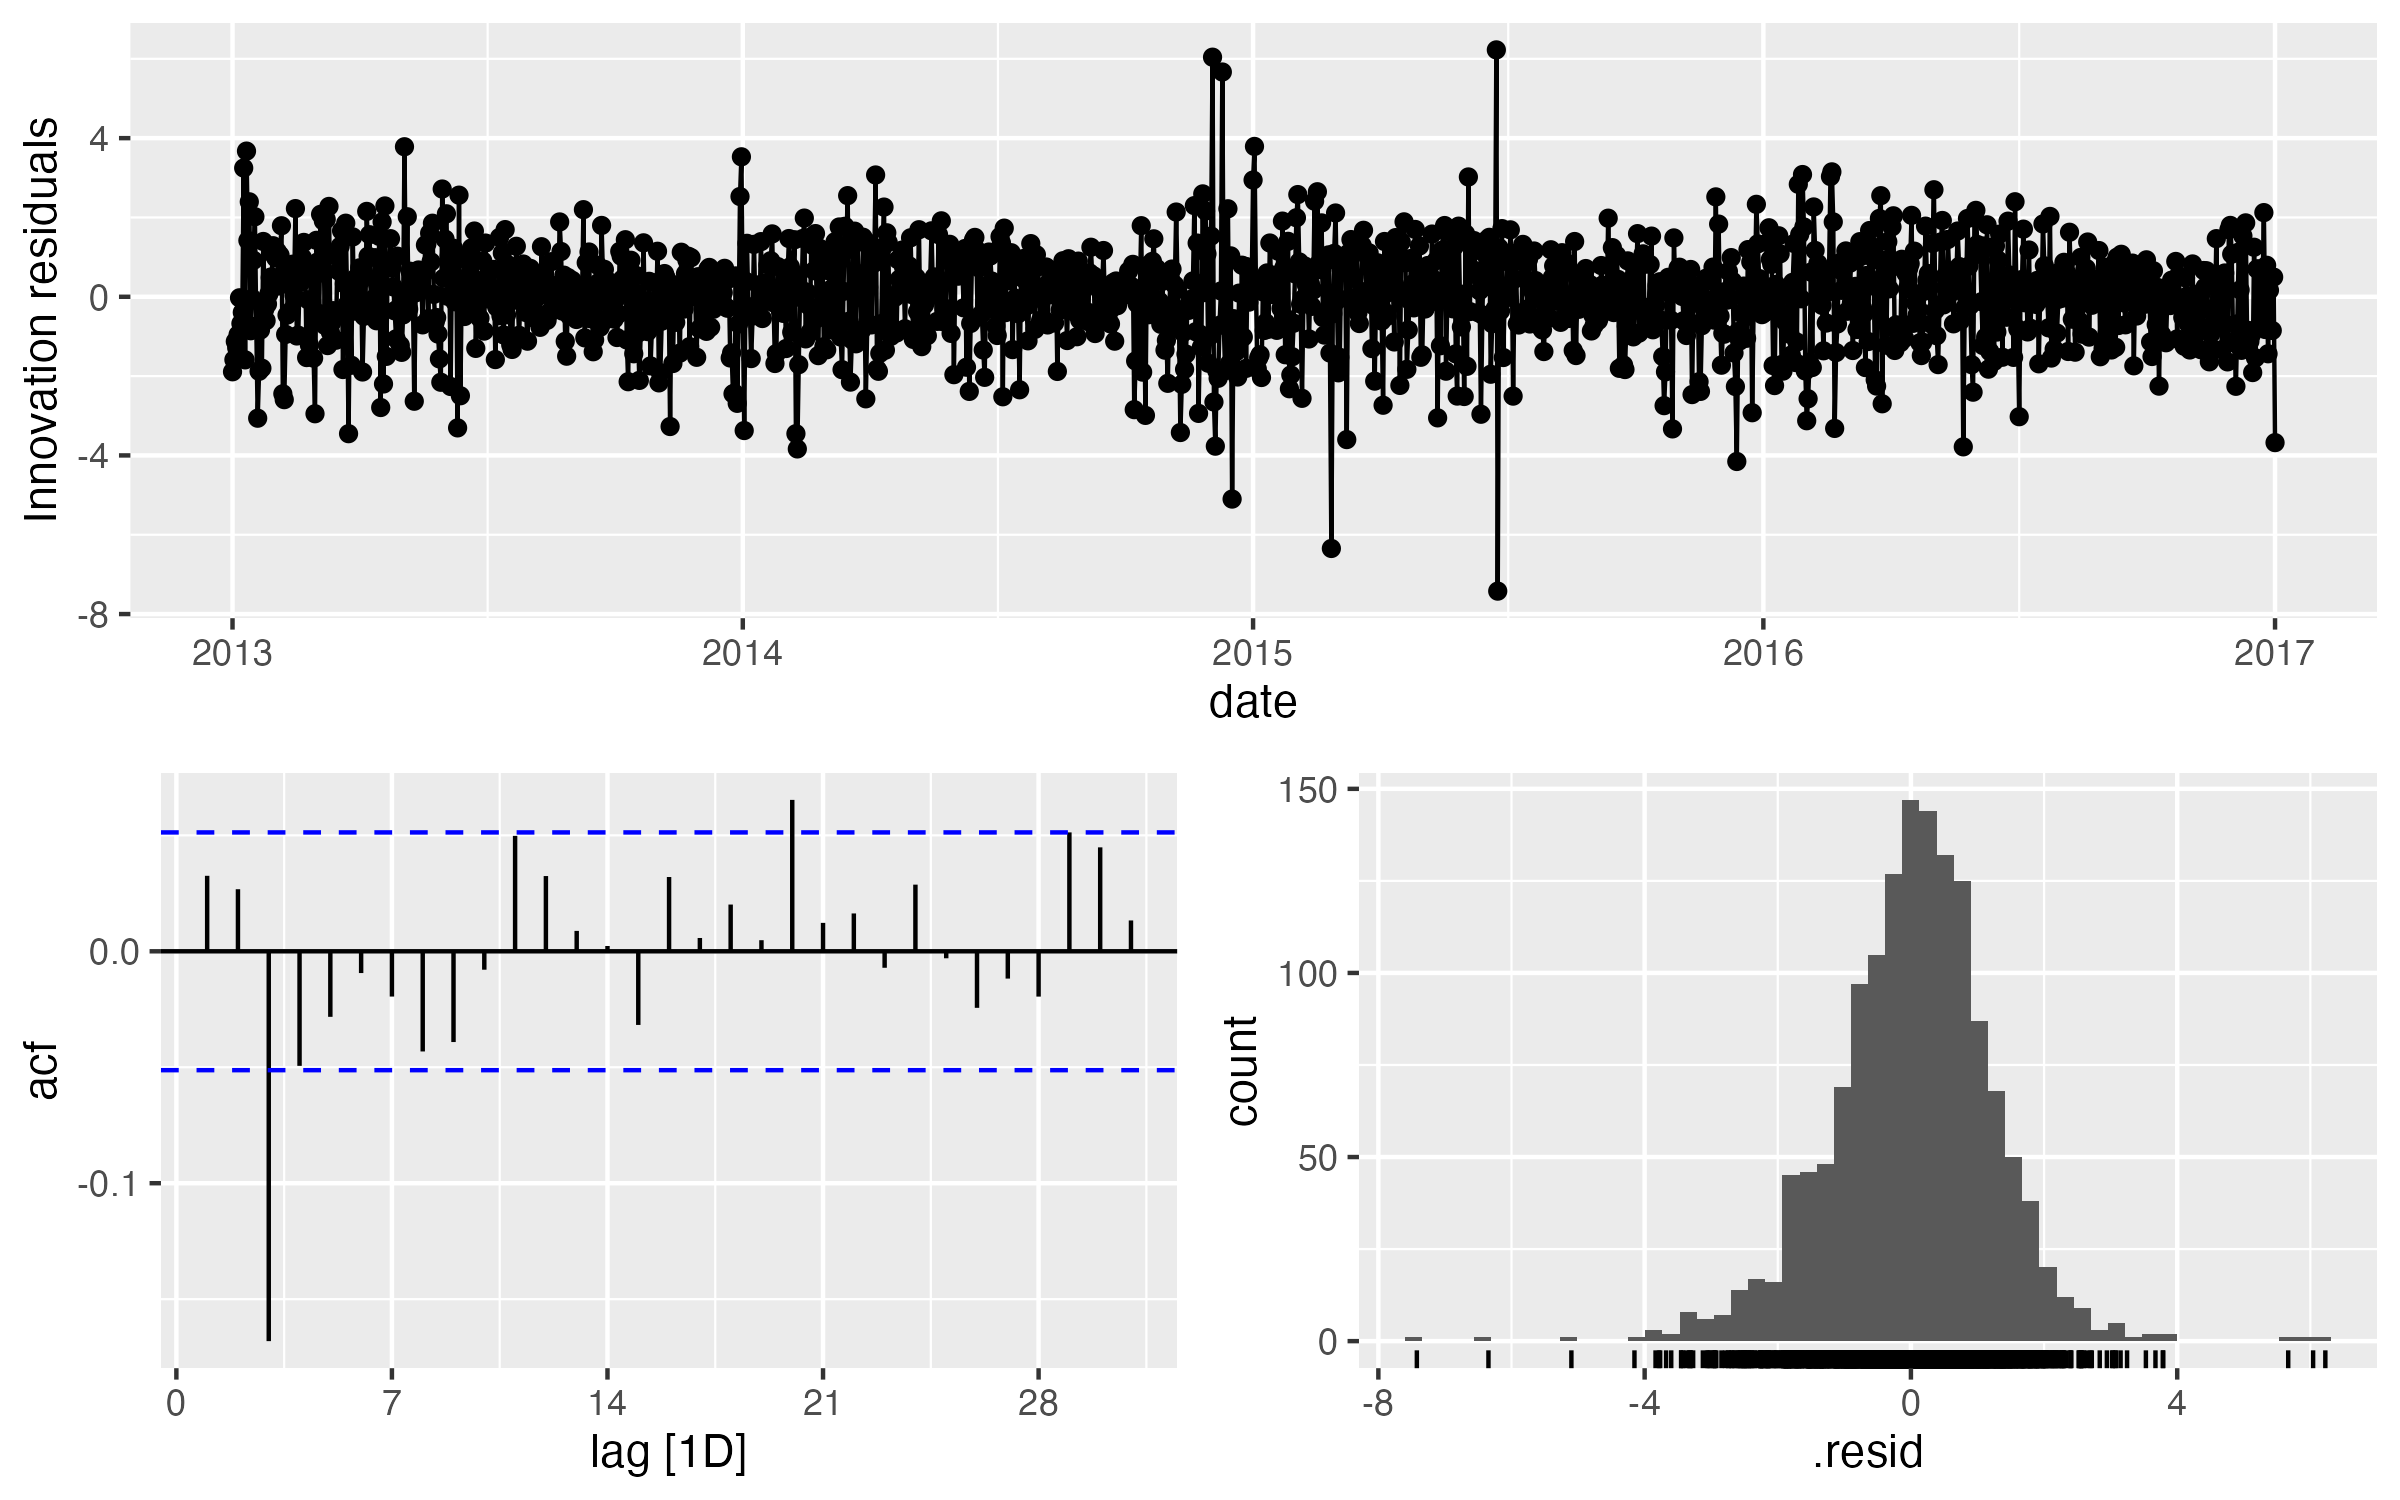
\includegraphics[width=.8\textwidth]{images/best_model_resid_diagnostic.png}
    \caption{\small \textit{Residual diagnostic plot for SARIMA with dummy variables}}
    \label{fig:figure1}
\end{figure}

\begin{figure}[!h]
    \centering
    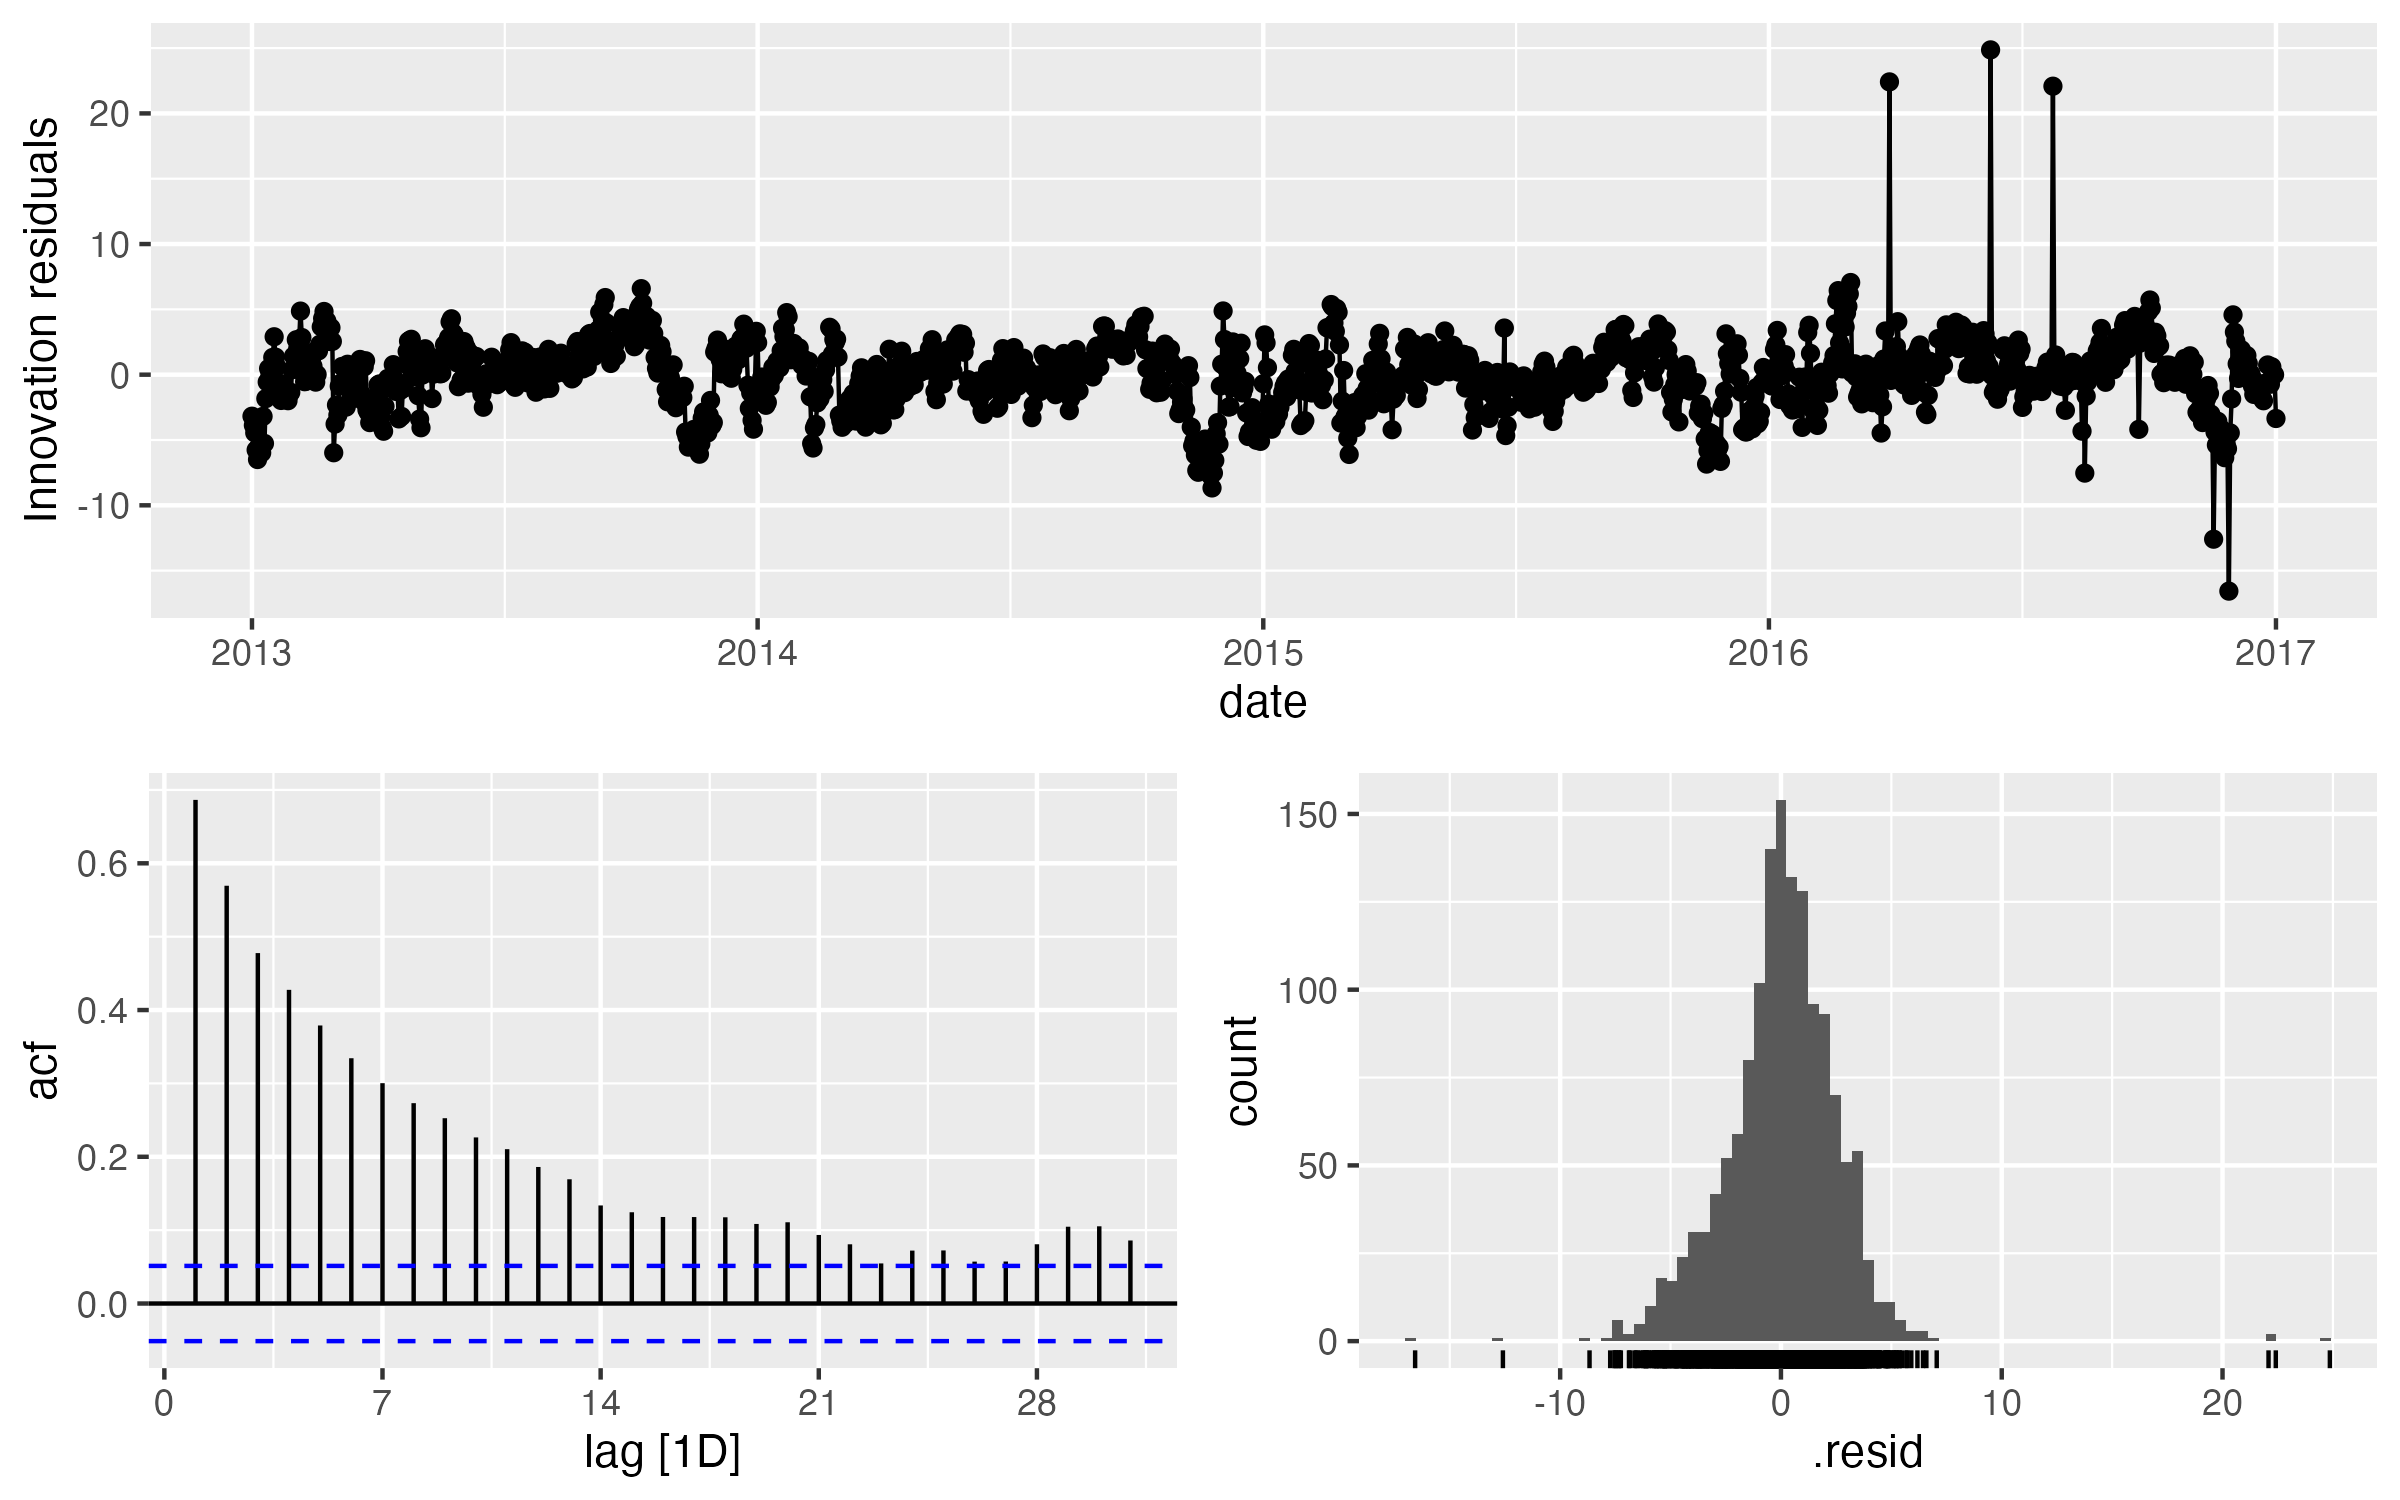
\includegraphics[width=.8\textwidth]{images/linear_dummy_model_resid_diagnostic.png}
    \caption{\small \textit{Residual diagnostic plot for standard linear model with dummy variables}}
    \label{fig:figure1}
\end{figure}






